\documentclass{beamer}
\usepackage{hyperref}
\usepackage{caption}
\usepackage[T1]{fontenc}
\usepackage[utf8]{inputenc}
\usepackage{lmodern}
\usepackage[english]{babel}
\linespread{1.25} %easier reading/grading.
\usepackage{amsmath} %d'oh
\usepackage{amsfonts}
\usepackage{graphicx}
\usepackage{bold-extra} %for \mb
\usepackage[margin=2.5cm]{geometry} %for custom margins
\usepackage{enumerate} %for special counters
\usepackage{titlesec} %for section numbering
\usepackage{ifthen}
\renewcommand\thesubsection{\alph{subsection}}
\titleformat{\section}{\it \bf \large}{{\normalfont  \bf \thesection.}}{4pt}{}[]
\titleformat{\subsection}{\it \bf \large}{{\normalfont \bf \quad \large  \thesection \thesubsection)}}{5pt}{}[]
\titleformat{\subsubsection}{\bf \it}{\qquad}{5pt}{}[]

\numberwithin{equation}{section}
\renewcommand{\O}{\mathcal{O}}
\renewcommand{\bf}{\bfseries}
\renewcommand{\sc}{\scshape}
\renewcommand{\it}{\itshape}
\renewcommand{\div}{\text{div }}
\renewcommand{\Re}{\mathbb{R}}
\newcommand{\op}{\left(}
\newcommand{\cp}{\right)}
\newcommand{\N}{\mathbb{N}}
\newcommand{\mb}{\mathbf}
\newcommand{\nn}{\\\nonumber}
\newcommand{\curl}{\text{curl }}
\newcommand{\inp}[2]{\left<#1, #2\right>}
\newcommand{\pdrv}[2][x]{\frac{\partial #2}{\partial #1}}

\title{Pricing of Barrier Options using Finite Difference}
\subtitle{For up-and-out options}
\author{Roel Deckers}

\begin{document}
  \begin{frame}
    \frame{\titlepage}
  \end{frame}
\begin{frame}{Barrier Options}
\begin{itemize}
\item{Barrier options are options which either come into play or expire worthelessly
if the underlying asset hits a predetermined value $B$.}
\item{{\em Up-an-out options} are which expire worthlessly when they exceed a certain barrier $B$.}
\end{itemize}
\end{frame}
\begin{frame}{Methodology}
  We start with the standard Black-Scholes equation for pricing options
  \begin{align}
    \label{eq:pde}
    \pdrv[t]V + rS\pdrv[S]V + \frac{1}{2}\sigma^2S^2\pdrv[S^2]{^2V}-rV = 0
  \end{align}
  and then discretize in $S$ space using a standard equidistant grid and the standard second-order central finite-difference methods for the derivatives.
\end{frame}

\begin{frame}{Methodology}
  \begin{align}
    \pdrv[S]V &= \frac{V(t, S+\Delta S)-V(t, S-\Delta S)}{2\Delta S},\nn
    \pdrv[S^2]{^2V} &= \frac{V(t,S+\Delta S)-2V(t,S)+V(t,S-\Delta S)}{\Delta S^2}
  \end{align}
\end{frame}

\begin{frame}{Methodology}
  We Discretize in time by making the change of variable $t\to \tau, \tau = T-t$ and integrate using the BDF-2 scheme.
  The BDF-2 scheme is given by
  \begin{align}
   &V^+ - \frac{4}{3}V + \frac{1}{3}V^- = \frac{2}{3}\Delta t A V^+\nn
   \to& \left(3I-2\Delta t A)V^+ = 4V-V^-
  \end{align}
  Where $A$ is a tridiagonal matrix constructed using the finite-difference scheme we showed before.
\end{frame}

\begin{frame}{Boundary Conditions}
  The boundary conditions on a up-and-out barrier option are given by
  \begin{align}
    V(S > \text{barrier}) = V(S < K) = 0.
  \end{align}
  This is easy to understand intuitively, as these are the conditions imposed on us by the definition of the barrier and the pay-off function respectively.
  %injection method
\end{frame}

\begin{frame}{Results}
    \centering
      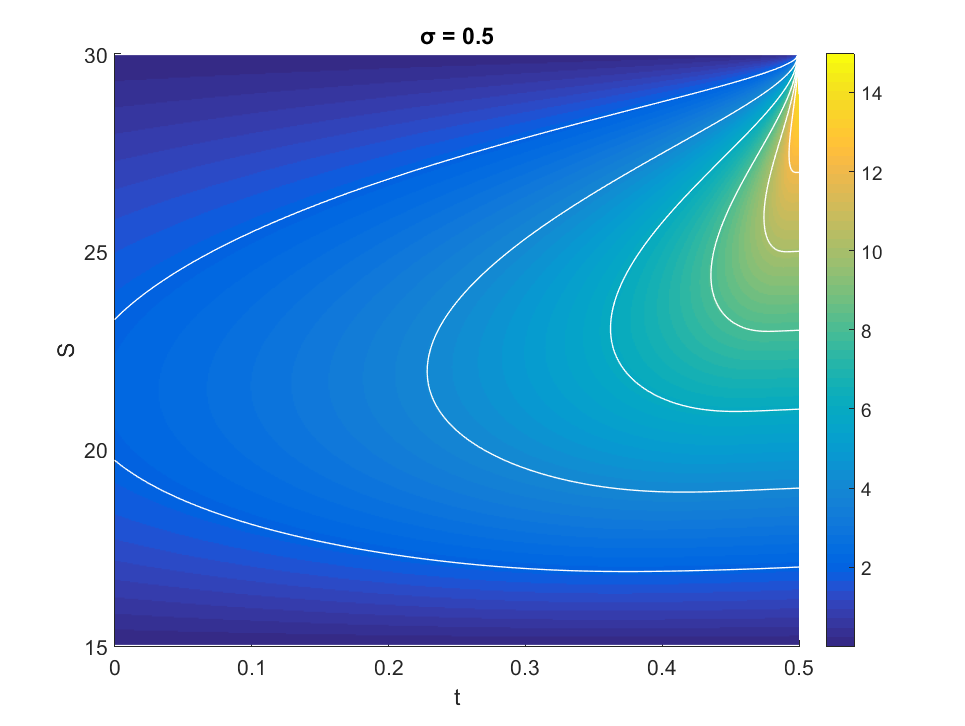
\includegraphics[width=1\textwidth]{../plots/field}
\end{frame}

\begin{frame}{Results}
    \centering
      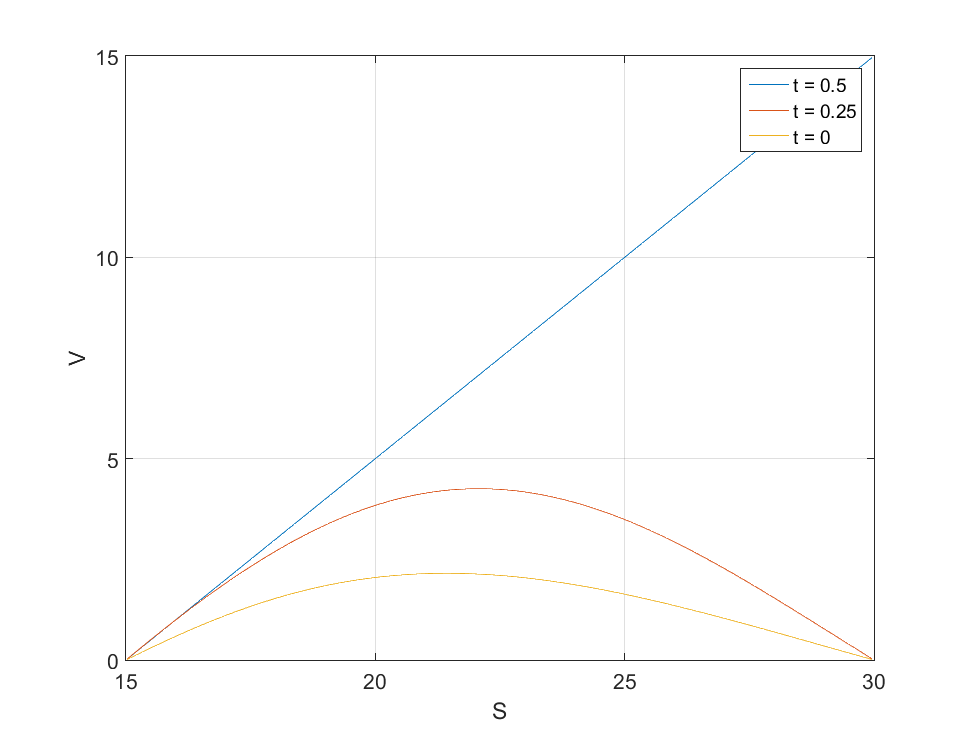
\includegraphics[width=1\textwidth]{../plots/lines}
\end{frame}

\begin{frame}{Results}
    \centering
      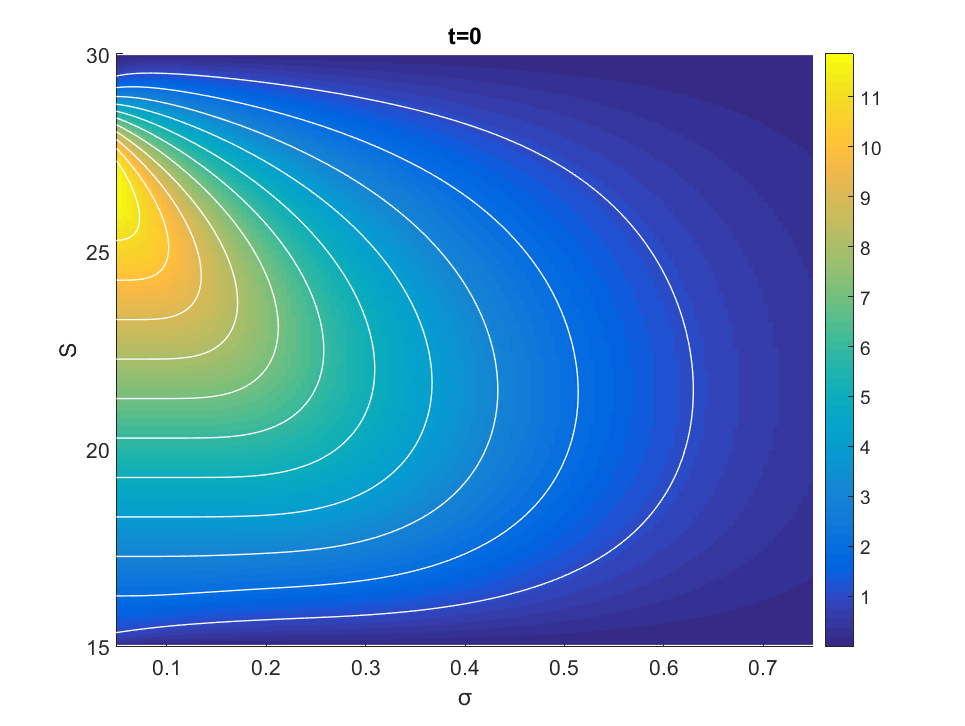
\includegraphics[width=1\textwidth]{../plots/sigma_field}
\end{frame}

\begin{frame}{Results}
    \centering
      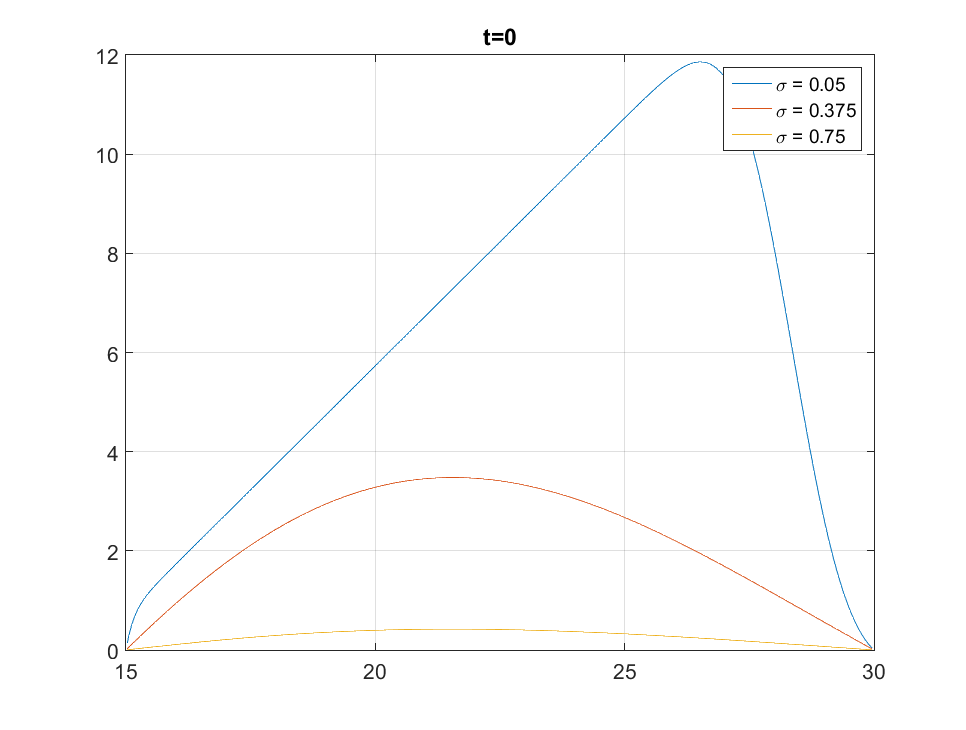
\includegraphics[width=1\textwidth]{../plots/sigma_lines}
\end{frame}

\begin{frame}{Greeks}
\begin{itemize}
  \item{$\Delta$ is a measure of the rate of change in the value $V$ as function of $S$. It is given by \Delta = \pdrv[S]V.}

  \item{$\nu$ (Vega) is a measure of how the value of an option changes with the implied volatility of the underlying asset. It is defined as $\nu = \pdrv[\sigma]{V}$.}
\end{itemize}
\end{frame}

\begin{frame}{$\Delta$}
\centering
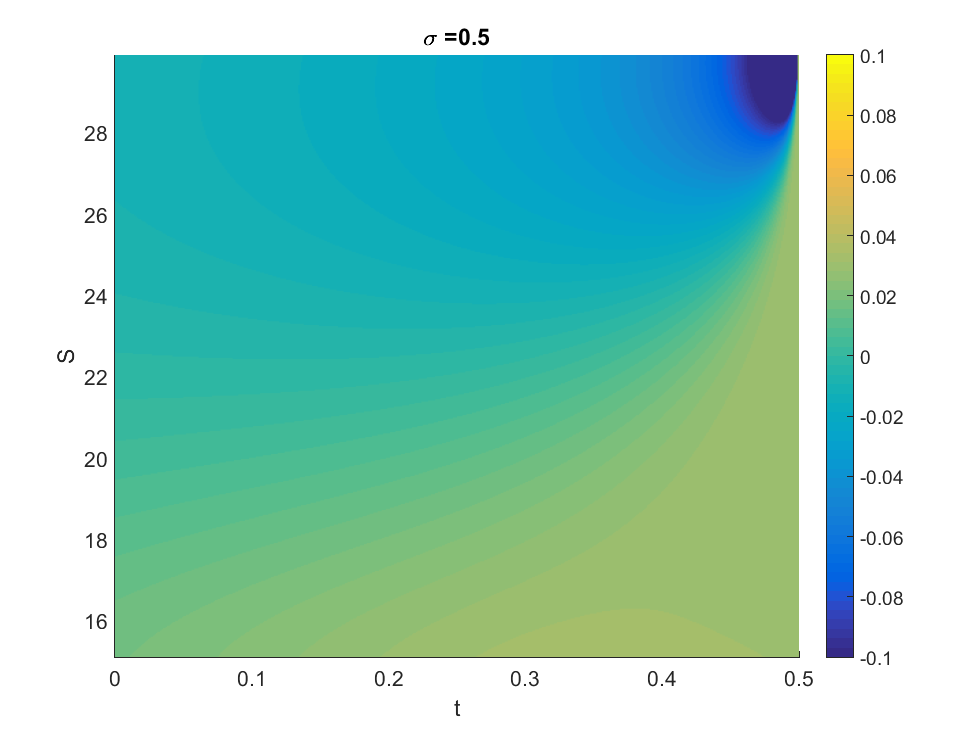
\includegraphics[width=1\textwidth]{../plots/delta_field}
\end{frame}

\begin{frame}{Results}
    \centering
      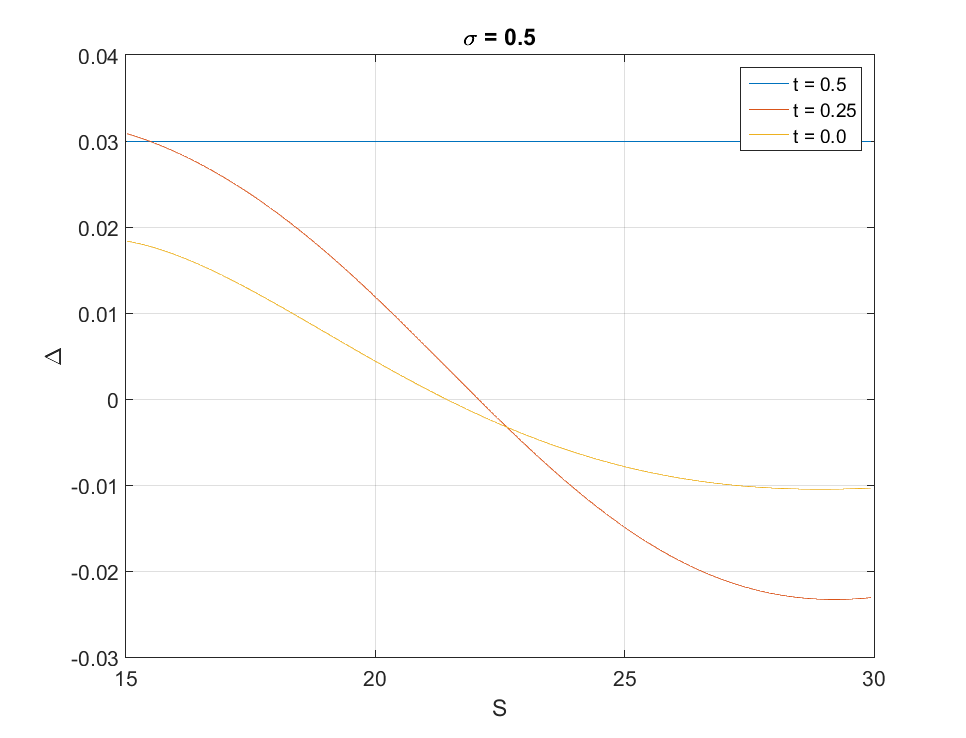
\includegraphics[width=1\textwidth]{../plots/delta_lines}
\end{frame}

\begin{frame}{$\Delta$}
\centering
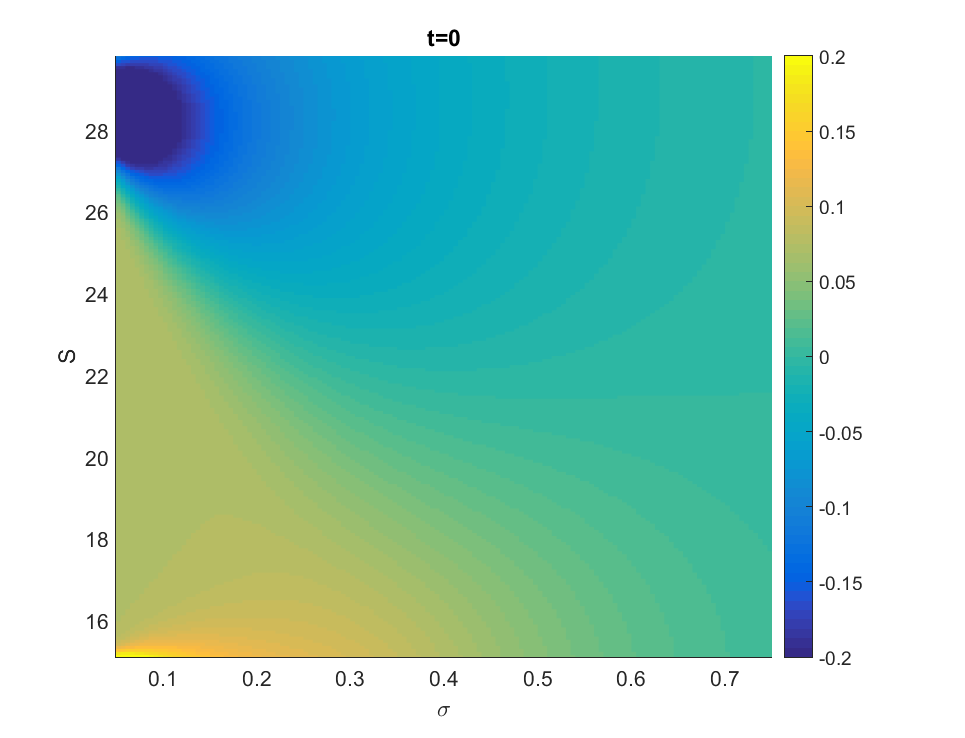
\includegraphics[width=1\textwidth]{../plots/delta_sigma_field}
\end{frame}

\begin{frame}{$\nu$}
  \centering
  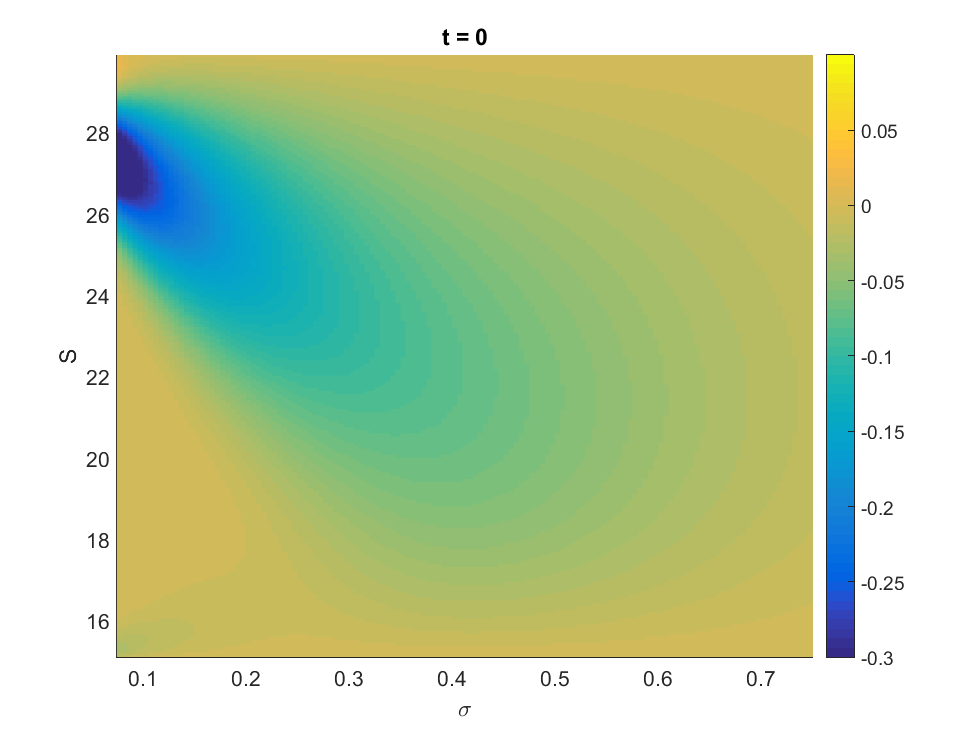
\includegraphics[width=1\textwidth]{../plots/vega_field_sigma}
\end{frame}

\begin{frame}

\end{frame}

\end{document}
